\documentclass{article}
\usepackage{graphicx}
\usepackage{float}
\usepackage[dvipsnames]{xcolor}
\usepackage{listings}
\usepackage{indentfirst}
\usepackage{paralist}

\lstset{numbers=left,framexleftmargin=10mm,frame=none,backgroundcolor=\color[RGB]{245,245,244},keywordstyle=\bf\color{blue},identifierstyle=\bf,numberstyle=\color[RGB]{0,192,192},commentstyle=\it\color[RGB]{0,96,96},stringstyle=\rmfamily\slshape\color[RGB]{128,0,0},showstringspaces=false}
\begin{document}
\title{\textbf{Design of rescue mode in the installer}}
\author{Tao Wu}
\date{\today}
\maketitle
\section{Introduction}
Rescue mode is a new feature designed for user to modify or repair already
installed operating systems. \\

For example, after you have completed the installation, you login the system and
do some changes like adding some network services or modifying some user
accounts, etc. However you might find that you happen to damage some system
configure files which causes your failing to boot again, meaning that you are
not able to access the system any more. That is where rescue mode can help.\\

By entering rescue mode, you can find the whole system mounted in a particular
path (by default, /mnt/sysimage), and you can modify or restore the damaged
configure files so that the system boot successfully again.\\

\section{The functions provides}
\begin{itemize}
\item Find out all systems located in all disks.
\item Online SCSI disk which might have system on it.
\item Mount the disk user selected to /mnt/sysimage for read-write or read-only.
\item Invoke a shell for user to work on.
\end{itemize}

\section{How to verify the result?}

\noindent
\textbf{Test Steps:}\\
\noindent
1. Start the installer from ftp or live CD.\\
2. At the initial screen, select `Rescue Mode'.\\
\begin{figure}[H]        
\center{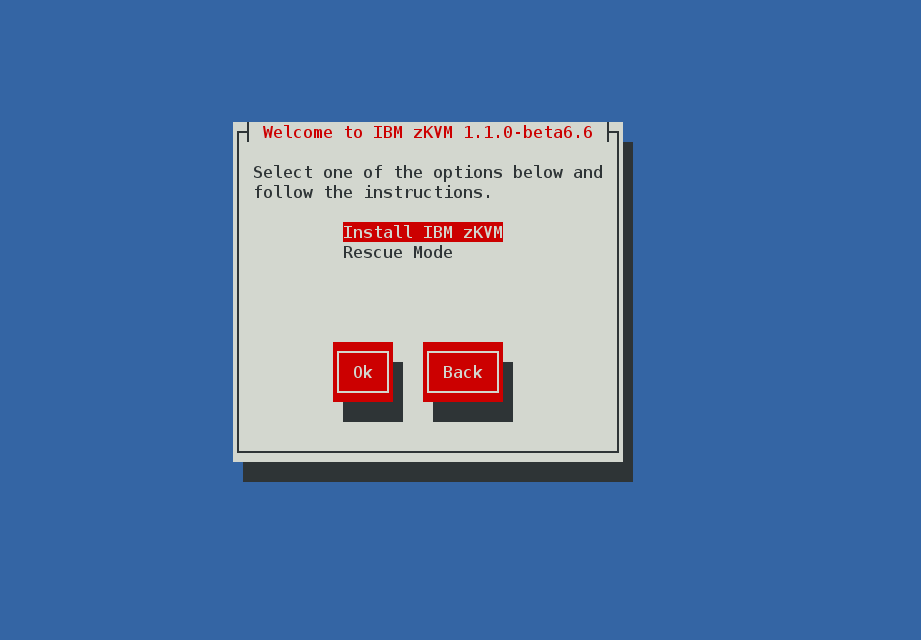
\includegraphics[width=\textwidth]  {boot_rescue.png}}        
%\caption{\label{fig:my-label} My figure.  An example of a cool figure}      
\end{figure}
\noindent
3. When prompted, direct installer to scan your disks for existing
installations by clicking the `Continue' button.\\
\begin{figure}[H]        
\center{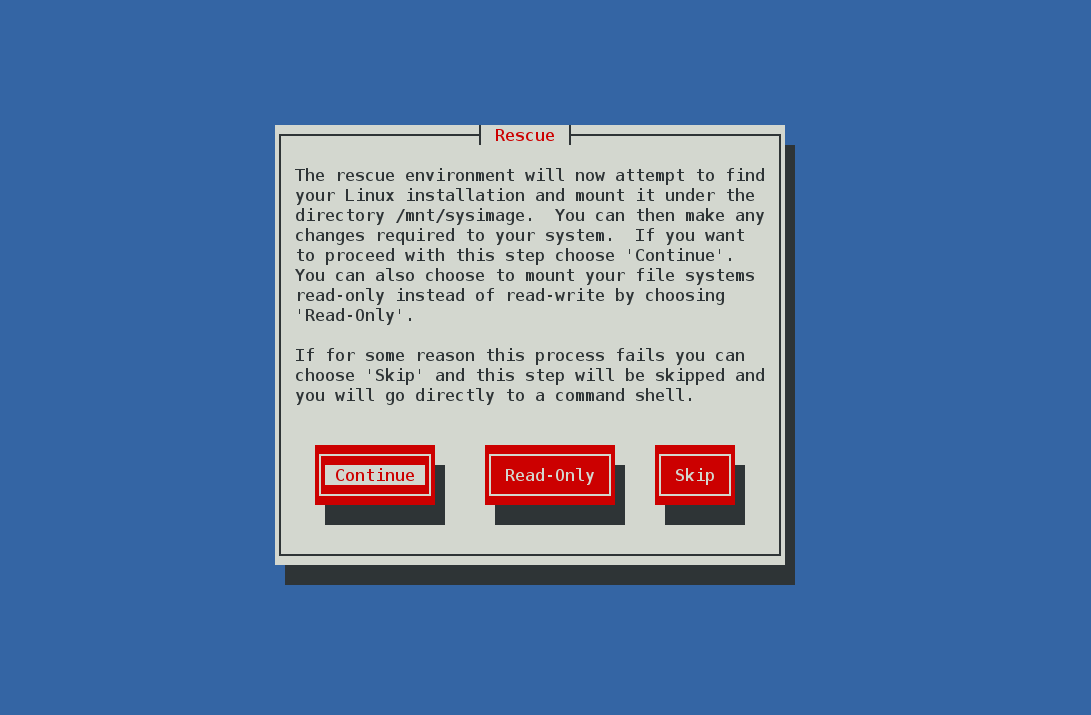
\includegraphics[width=\textwidth]  {rescue_prompt.png}}        
\end{figure}
\noindent
4. Add a SCSI disk through the `Add zFCP' button if you want to.\\
\begin{figure}[H]        
\center{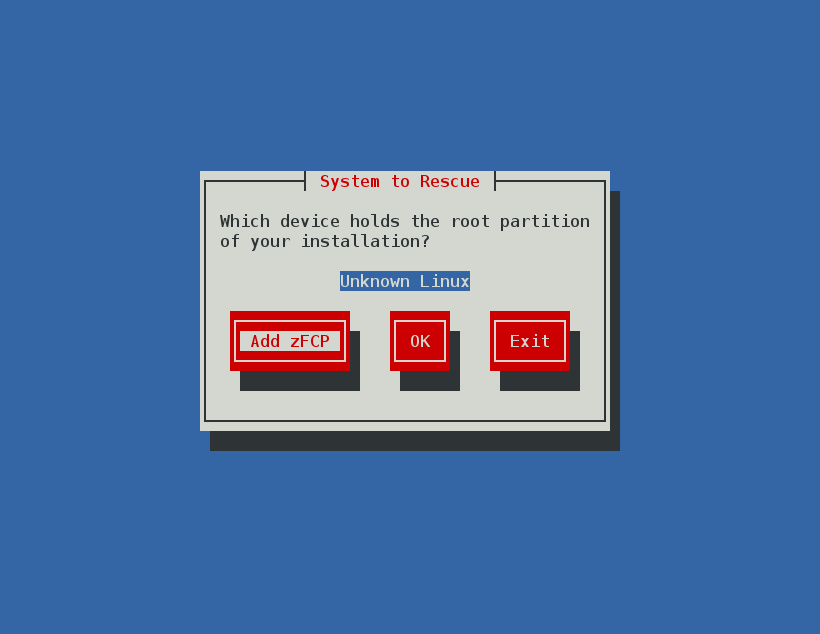
\includegraphics[width=\textwidth]  {list_system.png}}        
\center{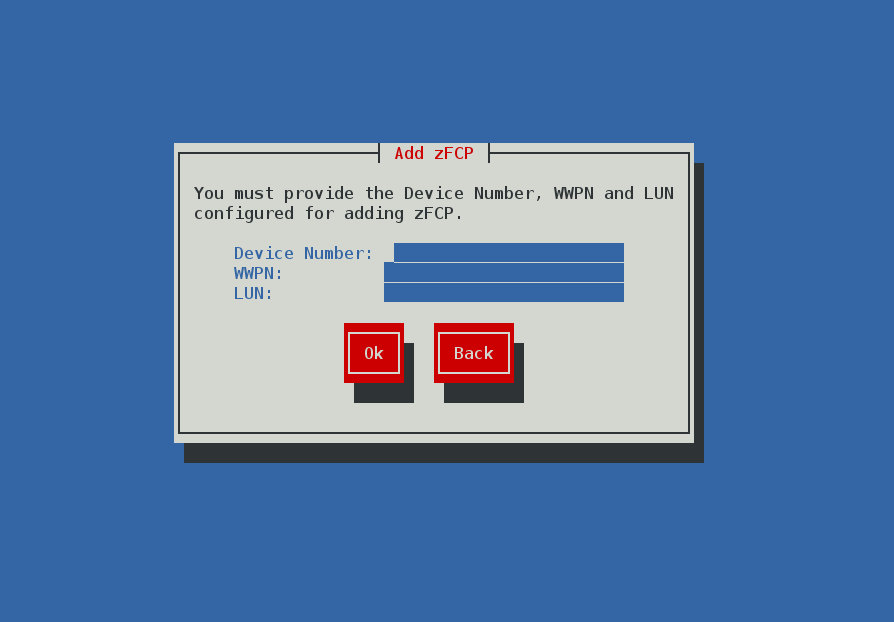
\includegraphics[width=\textwidth]  {add_zfcp.png}}        
\end{figure}
\noindent
5. Select OK and chroot into /mnt/sysimage for your existing installation.\\
\begin{figure}[H]        
\center{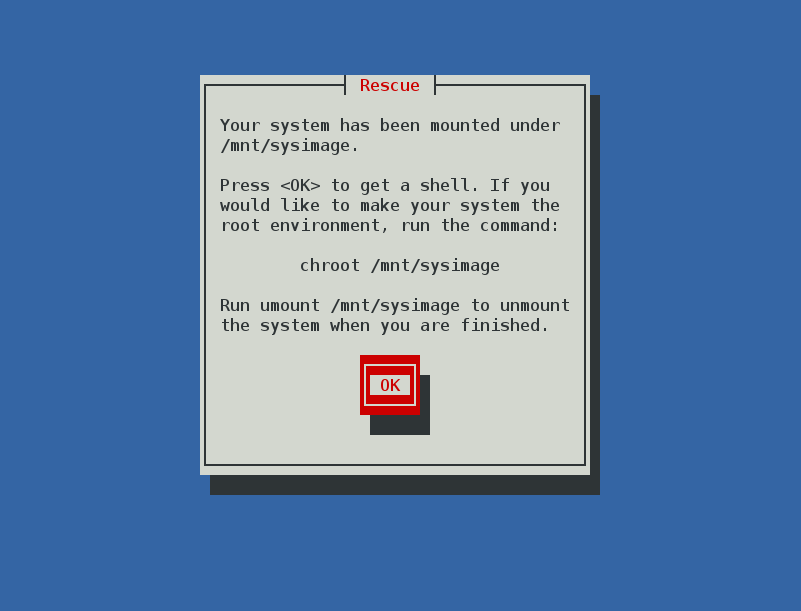
\includegraphics[width=\textwidth]  {mount_prompt.png}}        
\center{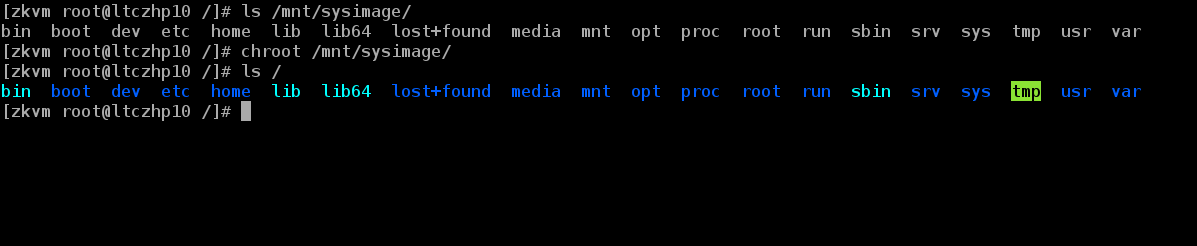
\includegraphics[width=\textwidth]  {ls_sysimage.png}}        
\end{figure}
\noindent
\textbf{Expected Results:}\\
\noindent
1. Installer should start and proceed to disk scan prompt.\\
2. Scanning your disk for existing installations should not result in a
failure.\\
3. Installer successfully online the SCSI disk if you have chosen `Add zFCP'.\\
4. Installer should be able to mount read-write and read-only installations.\\
5. Selecting OK will present you with a shell where you are able to see the
previous installation mounted under /mnt/sysimage.\\
6. Additionally, you may be able to execute chroot /mnt/sysimage without error.\\

\end{document}
